\begin{frame}
 \frametitle{Addition of Vectors}

  \begin{itemize}
    \item By adding representative displacement vectors: Triangle Rule
\only<2>{
\begin{figure}[h]
  \psfrag{A}{$A$}
  \psfrag{B}{$B$}
  \psfrag{C}{$C$}
  \psfrag{P}{$P$}
  \psfrag{Q}{$Q$}
  \psfrag{R}{$R$}
  \psfrag{u}{$\textbf{u}$}
  \psfrag{v}{$\textbf{v}$}
  \psfrag{uv}{$\textbf{u}+\textbf{v}$}
  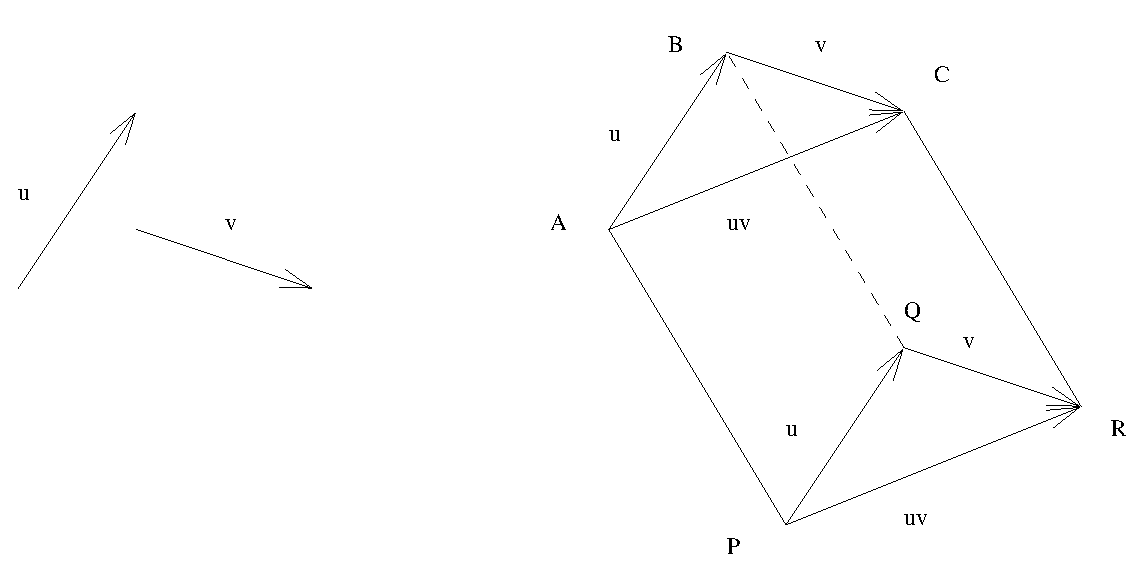
\includegraphics[height=1in]{../../modules/vectors/pictures/ok-vector_addition.eps}
  \label{fig:vector_addition}
  %\caption{Sum of two vectors}
\end{figure}}
    \item<3-> Properties:
    \begin{itemize}
      \item<4-> Commutative, $\textbf{u}+\textbf{v}$ = $\textbf{v}+\textbf{u}$ : Parallelogram Rule
\only<5, 10>{
\begin{figure}[h]
  \psfrag{A}{$A$}
  \psfrag{B}{$B$}
  \psfrag{C}{$C$}
  \psfrag{D}{$D$}
  \psfrag{u}{$\textbf{u}$}
  \psfrag{v}{$\textbf{v}$}
  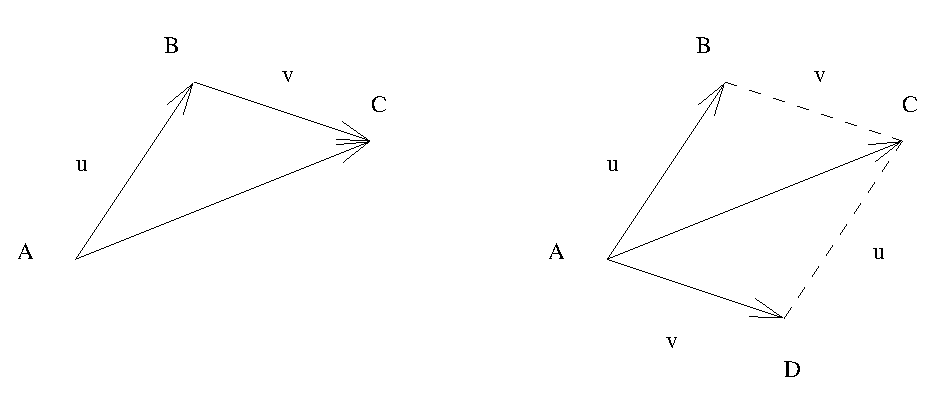
\includegraphics[height=1in]{../../modules/vectors/pictures/ok-tri-para_rules.eps}
  \label{fig:tripara_rules}
  %\caption{Triangle and Parallelogram Rules}
\end{figure}}

      \item<6-> Associative, $(\textbf{u}+\textbf{v})+\textbf{w} = \textbf{u}+(\textbf{v}+\textbf{w})$ \\
      Extends addition to $\textbf{u}+\textbf{v}+\textbf{w}$
\only<7>{
\begin{figure}[h]
  \psfrag{A}{$A$}
  \psfrag{B}{$B$}
  \psfrag{C}{$C$}
  \psfrag{D}{$D$}
  \psfrag{u}{$\textbf{u}$}
  \psfrag{v}{$\textbf{v}$}
  \psfrag{w}{$\textbf{w}$}
  \psfrag{uv}{$\textbf{u}+\textbf{v}$}
  \psfrag{vw}{$\textbf{v}+\textbf{w}$}
  \psfrag{uvw}{$\textbf{u}+\textbf{v}+\textbf{w}$}
  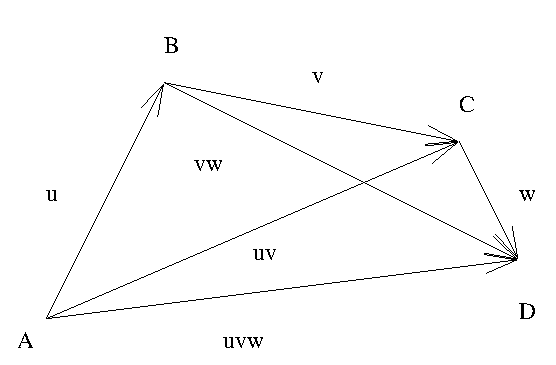
\includegraphics[height=1.5in]{../../modules/vectors/pictures/ok-assoc_addition.eps}
  \label{fig:assoc_adition}
  %\caption{Sum of three vectors}
\end{figure}}

      \item<8-> Opposite vector: If $\textbf{u}=\textbf{AB}$, then $\textbf{AB} + \textbf{BA} = \textbf{0}$,
      hence $\textbf{BA} = -\textbf{u}$.
    \end{itemize}
    \item<9-> Difference of vectors: $\textbf{u}-\textbf{v} = -\textbf{v}+\textbf{u}\textbf{}$: Parallelogram rule.

  \end{itemize}

\end{frame}